\documentclass{boi2014}

\usepackage{enumitem}
\usepackage{todonotes}

\renewcommand{\DayNum}{0}
\renewcommand{\TaskCode}{network}
\renewcommand{\TaskName}{Computer network}

\begin{document}

    There are $N$ computers in the computer classroom of a local
    secondary school and they are connected with cables to form
    a single network. Each cable joins two distinct computers.
    Some pairs of computers may not be joined by a
    cable, but a message sent from any computer could reach
    any other by travelling through computers joined by cables.
    A message always chooses the shortest route to travel:
    the number of \emph{intermediate} computers along its path
    (i.e. computers other than the sender and the receiver that
    the message visits) is minimised.
    
    Adam and Billy, who use distinct computers $x$ and $y$
    in this classroom, wish to determine a shortest route
    between their computers.

    They do not know the layout of the cables but they can
    send messages between all pairs of computers and calculate
    the number of intermediate computers that they visit.

    However, Adam and Billy are not very good with computers
    and they ask for your help to achieve their goal without sending
    too many messages.

    \Task
    Find a shortest route between computers $x$ and $y$ without
    sending more messages than is allowed.

    \Implementation
    You need to implement one procedure \method{findRoute(N, x, y)} that
    takes the following parameters:

    \begin{itemize}
        \item $N$ --- the number of computers in the classroom
            (they are labelled from $1$ to $N$)
        \item $x, y$ --- the labels of Adam and Billy's computers
            ($x \neq y$ and $1 \le x, y \le N$)
    \end{itemize}

    Your procedure \method{findRoute} can call function \method{ping(i, j)}
    that takes as parameters two distinct labels of computers
    ($i \neq j$ and $1 \le i, j \le N$) and returns the number of intermediate computers
    that a message travelling from $i$ to $j$ would visit.

    Your procedure \method{findRoute} has to describe a shortest route
    that a message sent from $x$ to $y$ might take. This must be done by
    repeatedly calling procedure \method{travelTo(k)} that takes as
    parameter the label of computer to which the message should travel
    next ($1 \le k \le N$). The message starts at $x$, and whenever
    \method{travelTo(k)} is called, it moves to computer $k$.

    In addition to the standard requirements (time and memory
    limits, no runtime errors), your submission has to achieve the following
    in order to solve a testcase:

    \begin{itemize}
        \item the message must be at $y$ when procedure \method{findRoute}
            terminates,
        \item any two consecutive computers in its path must be joined
            by a cable,
        \item it must take a shortest route,
        \item the number $M$ of calls to function \method{ping} must not
            exceed the allowed limit (see section Scoring),
        \item function \method{ping} and procedure \method{travelTo} must
            only be called with allowed parameter values.
    \end{itemize}

    \Example
    Consider the example shown in the diagram below (points correspond to
    computers, lines --- to cables). There are $N = 4$ computers in total,
    and Adam and Billy are using computers $x = 1$ and $y = 4$.

    \begin{wrapfigure}[1]{r}{5cm}
        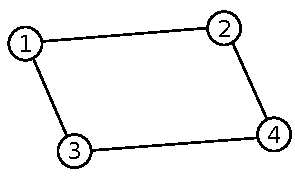
\includegraphics{network-example}
    \end{wrapfigure}

    The first call will be to procedure
    \begin{figure}[H]
        \centering
        \method{findRoute(4, 1, 4)}.
    \end{figure}

    Its sample behaviour could be as follows:

    \begin{figure}[H]
        \centering
        \method{ping(1, 4)} is called and returns $1$, \\
        \method{ping(1, 2)} is called and returns $0$, \\
        \method{ping(2, 4)} is called and returns $0$.
    \end{figure}

    This information is sufficient to determine that $1 \to 2 \to 4$ is a
    shortest route from $1$ to $4$. This should be described as follows:

    \begin{figure}[H]
        \centering
        \method{travelTo(2)} is called, \\
        \method{travelTo(4)} is called, \\
        \method{findRoute} terminates.
    \end{figure}

    \Scoring
    In all subtasks the constraint $2 \le N \le 1000$ holds.

    \begin{description}

        \item[Subtask 1 (25 points):] between
            any two computers there is exactly one shortest route; $M$
            cannot exceed $2N$.
        \item[Subtask 2 (25 points):] $M$ cannot exceed $N^2$.
        \item[Subtask 3 (25 points):] $M$ cannot exceed $4N$.
        \item[Subtask 4 (25 points):] $M$ cannot excced $2N$.
    \end{description}

    \Constraints
    \begin{description}
        \item[Time limit:] 1 s
        \item[Memory limit:] 64 MB
    \end{description}

    \Experimentation
    The sample grader on your computer will read data from standard input.
    The first line of input should contain four integers $N, x, y$ and the
    allowed limit for $M$. The next $N$ lines should
    contain $N$ integers each, describing the layout of the cables:
    the $j$--th integer in the $i$--th of these rows ($i \neq j$) should be
    the number of intermediate computers that a message sent from $i$ to $j$
    would visit. It does not matter what the entries with $i = j$ are.

    The following input describes the above example with $M$ limited by
    $100$:

    \begin{tabular}{p{\textwidth/3}p{\textwidth/3}p{\textwidth/3}}
        & \includefile{network.2-01p.in} &
    \end{tabular}

\end{document}

